\documentclass[french]{standalone}
\usepackage{babel}
\usepackage{tkz-fct}
\usepackage{tkz-euclide}
\usepackage{color}
\usepackage{numprint}

\renewcommand*\familydefault{\sfdefault}
\usepackage{sansmath}
\sansmath
\definecolor{gray75}{gray}{0.75}

\begin{document}
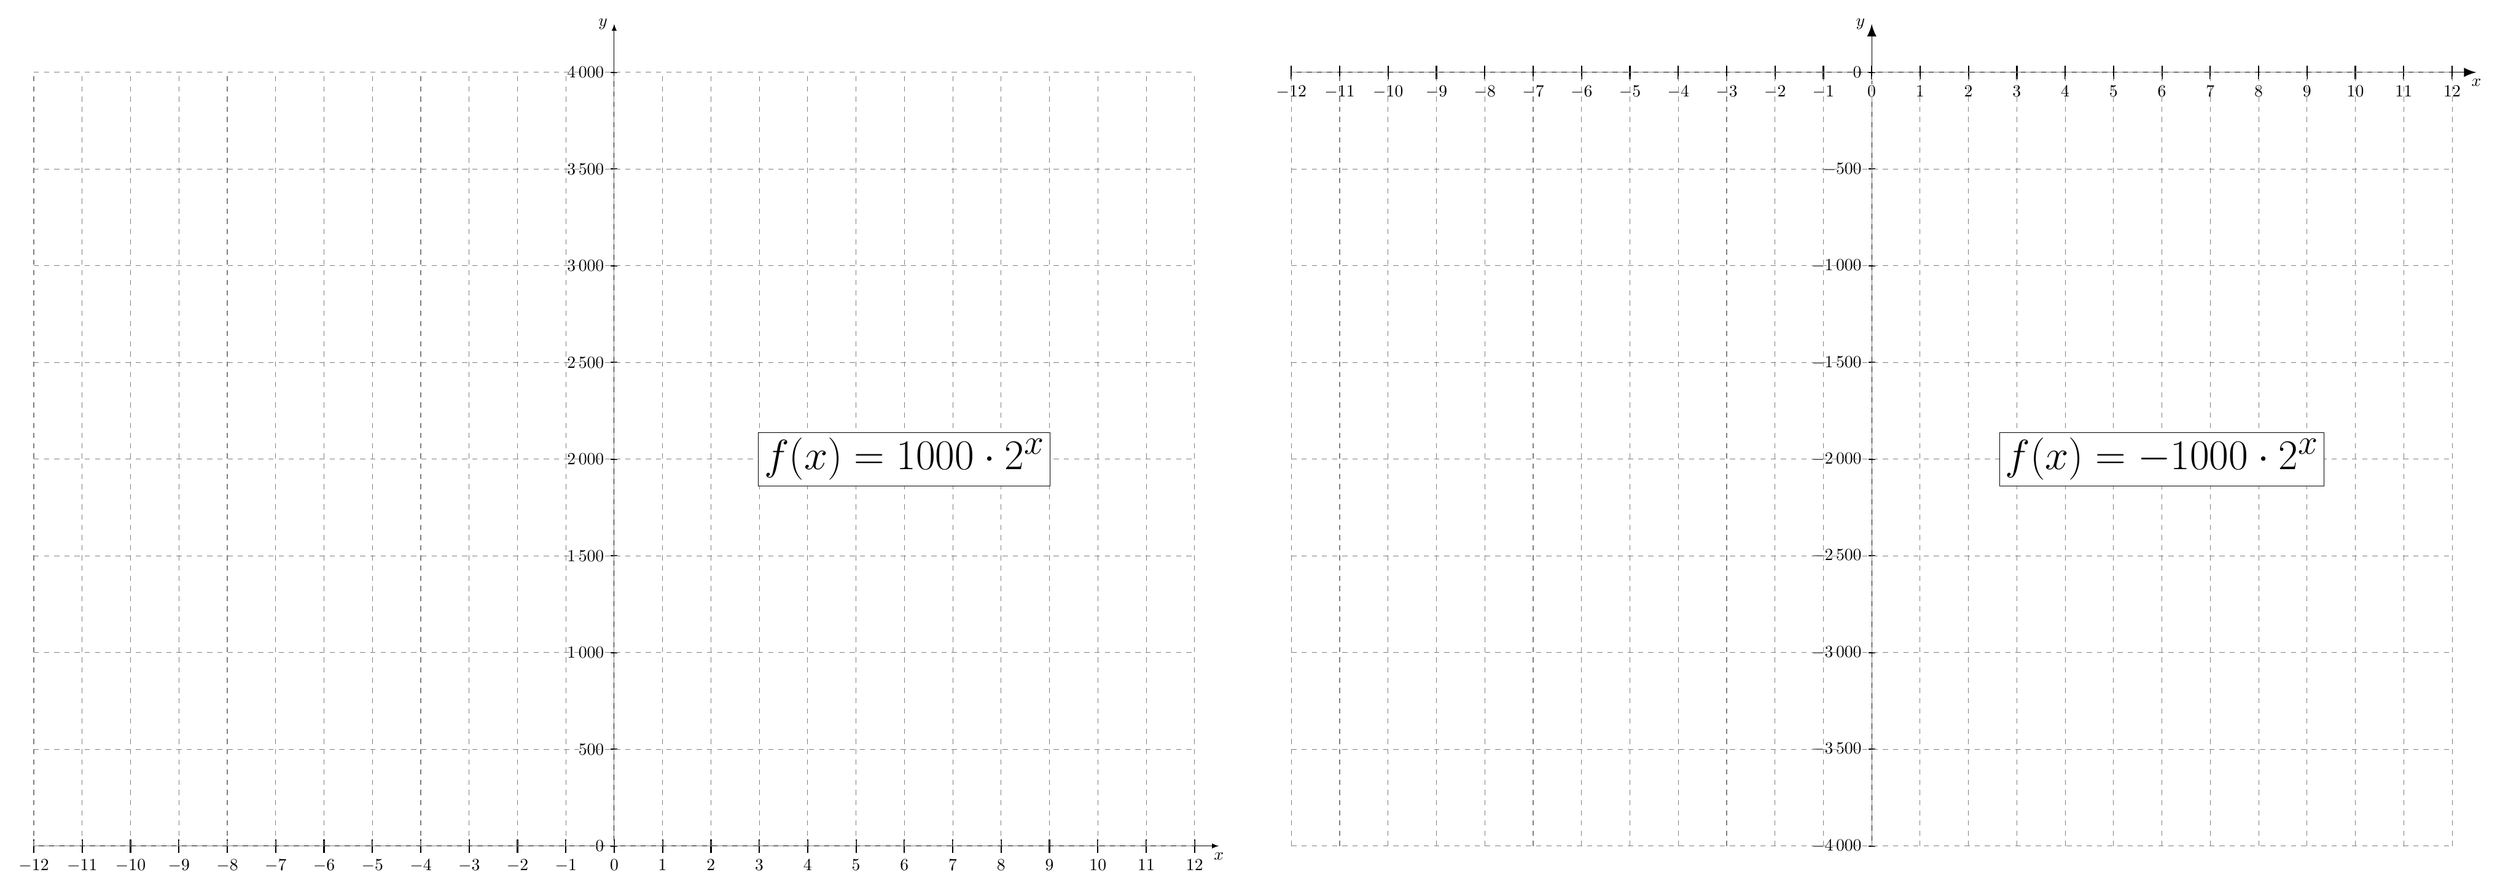
\begin{tikzpicture}[yscale=2, xscale=1]
\tkzInit[xmin=-12,xmax=12,ymin=0,ymax=4000, ystep=500, xstep=1]
\tkzAxeY
\tkzDrawX
\tkzLabelX
   \begin{scope}[dashed]
     \tkzGrid
   \end{scope}
   \tkzFct[domain=-12:2,line width=1.5pt]{(1000*exp(0.69314718056*x))}
      \tkzText[draw,fill=white](6,2000){\Huge$f(x)=1000\cdot 2^{x}$}

\begin{scope}[xshift=26cm, yshift=8cm]
  \tkzInit[xmin=-12,xmax=12,ymin=-4000,ymax=0, ystep=500, xstep=1]
\tkzAxeY
\tkzDrawX
\tkzLabelX

   \begin{scope}[dashed]
     \tkzGrid
   \end{scope}
   \tkzFct[domain=-12:2,line width=1.5pt]{(-1000*exp(0.69314718056*x))}
   \tkzText[draw,fill=white](6,-2000){\Huge$f(x)=-1000\cdot 2^{x}$}

\end{scope}
\end{tikzpicture}
\end{document}
